\documentclass{article}
\usepackage{blindtext}
\usepackage{multicol}
\usepackage{graphicx}
\usepackage{float}
\graphicspath{ {.} }

\title{Automatic GeoGuesser}
\author{Steel City Data Products}
\date{ALL WORK PROPOSED AND FOR INTERNAL USE ONLY}

\begin{document}
	\maketitle
	
	ABSTRACT - GeoGuesser is a popular web-based single-player game in which the play is given a particular location sourced from the Google Maps library. The goal is determine where, based on the available street-view to select the correct location on a political map. There are variations on this theme; the one we will focus on here is the instance where a user is given a single image from the street view. In this draft we will establish an architecture that will result in an architecture of an agent capable of mapping the images to the country from which they were taken. 
	
	\begin{multicols}{2}
	\section{Introduction}
	\subsection{GeoGuesser}
	As given by the website, geoguessr.com, "GeoGuesser is a geography game which takes you on a journey around the world and challenges your ability to recognize your surroundings." Indeed, the game functions by pulling in a section of StreetView from GoogleMaps, and challenging the player to select, on a political GoogleMap, the location that they have been given.
		
		\begin{figure}[H]
			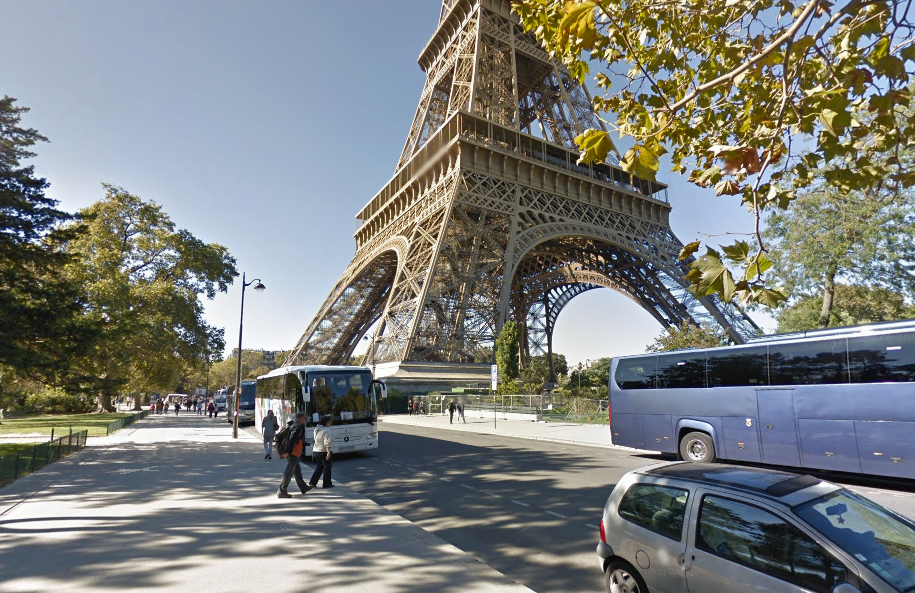
\includegraphics[width = 0.45\textwidth]{eiffeltourpic.png}
			\caption{A user may be given a view from StreetView of a location...}
		\end{figure}
		
		\begin{figure}[H]
			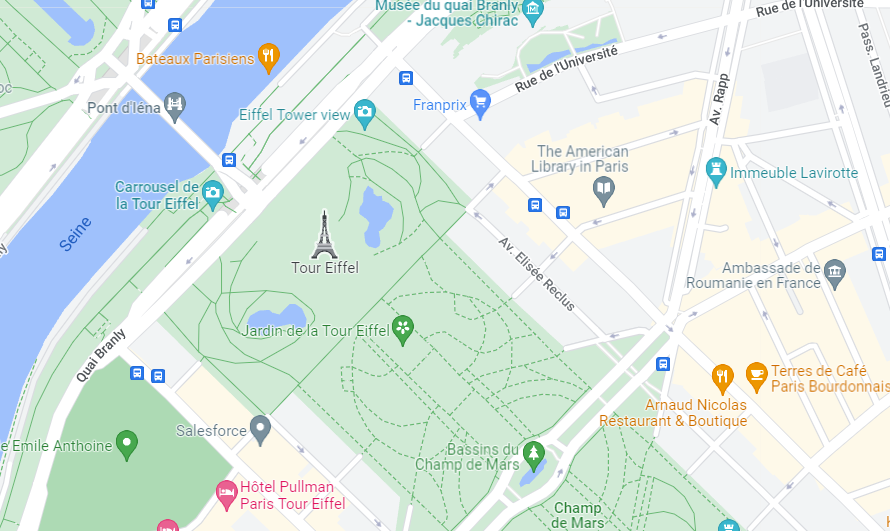
\includegraphics[width = 0.45\textwidth]{eiffeltourmap.png}
			\caption{... and need to guess as to where the are based on what they can see around them.}
		\end{figure}
		
		
	
	Some locations, like the one shown, will be readily identified. However, as the locations can be anywhere in the world (constrained by only the availability of GoogleMaps for a location) this become a much more difficult process. 
	
	\subsection{High-Level Precision}
	Some players have developed a vast repertoire of skill for accomplishing this task, even in the most difficult of circumstances. Variation of the base game include only seeing part of the screen, or only seeing the screen for an extreme short time (as little as 0.1 sec.) But still they are able to achieve high levels of consistent accuracy with their 'GeoGuesses'. 
	
	\subsection{Features}
	In order to achieve such startling results, player utilize a variety of clues that can be found in the picture they are given as a hint. This section will describe and give examples.
	
	\subsubsection{Soil}
	\subsubsection{Signs}
	\subsubsection{Plants}
	\subsubsection{License Plates}
	\subsubsection{Poles}
	\subsubsection{Roads}
	\subsubsection{Automobiles}
	\subsubsection{Image Capture Anomalies}
	
	\section{Architecture}
	
	We will seek to mimic the the way that high-level players operates. We will construct an ensemble model, which a component for each of the features mentioned previously. 
	The first part of this will comprise of a Detection module. This will be the part of the module that is tasked with identifying the particular features (ie. poles, license plates).
	After this, there will be a module that is responsible for determining the location of the picture. This will be based off of the excerpted piece of the photo that has been determined to be the object of the desired feature. This will be termed the Localization Model. 
	Each feature will have a twin set of modules that then will cast a confidence-weighted vote, along side other Detection-Localization Pairs, to result in a final determination. A schematic of this architecture is given in Figure 3
	
	\begin{figure*}
		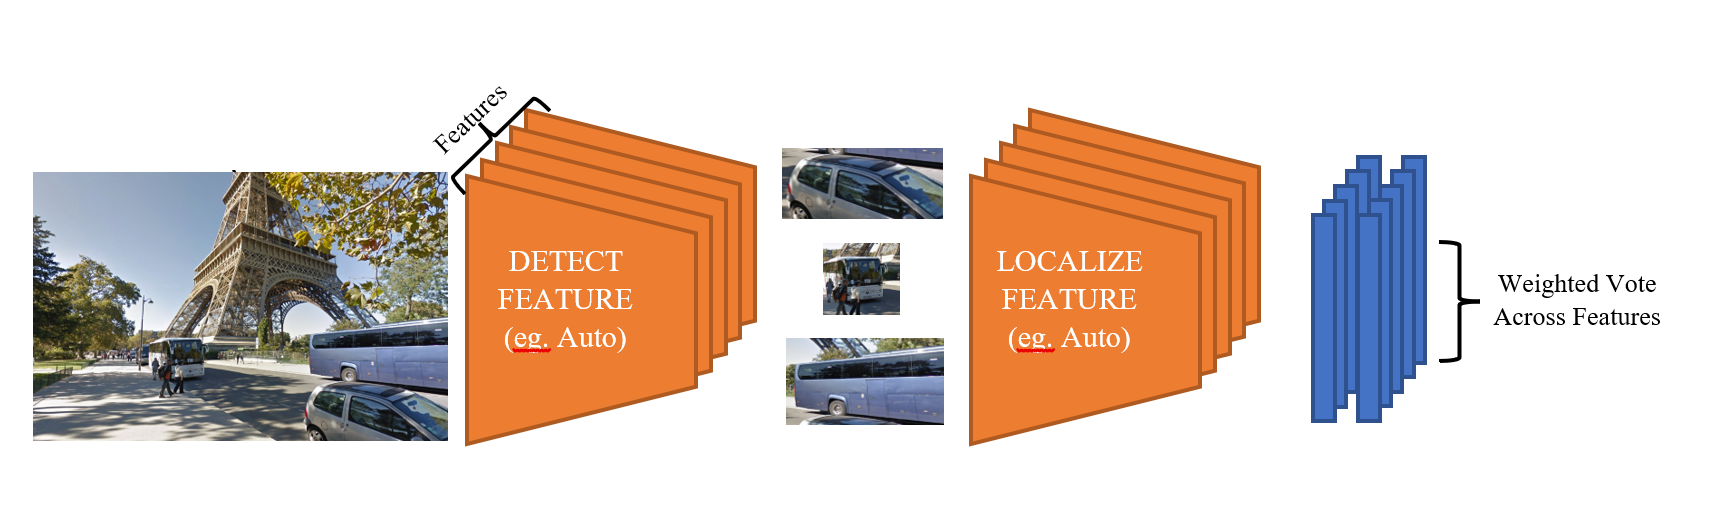
\includegraphics[width=\textwidth]{architecture.png}
		\caption{Proposed Architecture}
	\end{figure*}






	\end{multicols}
	
\end{document}